%%%%%%%%%%%%%%%%%%%%%%%%%%%%%%%%%%%%%%%%%
% Thesis Presentation
% Software Defined Total Power Radiometer
% Version 0.3
% Matthew E. Nelson
% Iowa State University
% 
% License:
% CC BY-NC-SA 3.0 (http://creativecommons.org/licenses/by-nc-sa/3.0/)
%
%%%%%%%%%%%%%%%%%%%%%%%%%%%%%%%%%%%%%%%%%

%----------------------------------------------------------------------------------------
%	PACKAGES AND THEMES
%----------------------------------------------------------------------------------------

%\documentclass{beamer}

%Uncomment this out and comment out the above to print out notes
\documentclass[notes]{beamer}

\mode<presentation> {

%Beamer Themes, uncomment the theme you wish to use

%\usetheme{default}
%\usetheme{AnnArbor}
\usetheme{Antibes}
%\usetheme{Bergen}
%\usetheme{Berkeley}
%\usetheme{Berlin}
%\usetheme{Boadilla}
%\usetheme{CambridgeUS}
%\usetheme{Copenhagen}
%\usetheme{Darmstadt}
%\usetheme{Dresden}
%\usetheme{Frankfurt}
%\usetheme{Goettingen}
%\usetheme{Hannover}
%\usetheme{Ilmenau}
%\usetheme{JuanLesPins}
%\usetheme{Luebeck}
%\usetheme{Madrid}
%\usetheme{Malmoe}
%\usetheme{Marburg}
%\usetheme{Montpellier}
%\usetheme{PaloAlto}
%\usetheme{Pittsburgh}
%\usetheme{Rochester}
%\usetheme{Singapore}
%\usetheme{Szeged}
%\usetheme{Warsaw}

%Beamer color themes, select one, or use none to use the themes default color scheme

%\usecolortheme{albatross}
\usecolortheme{beaver}
%\usecolortheme{beetle}
%\usecolortheme{crane}
%\usecolortheme{dolphin}
%\usecolortheme{dove}
%\usecolortheme{fly}
%\usecolortheme{lily}
%\usecolortheme{orchid}
%\usecolortheme{rose}
%\usecolortheme{seagull}
%\usecolortheme{seahorse}
%\usecolortheme{whale}
%\usecolortheme{wolverine}

% To remove the footer line in all slides uncomment this line
%\setbeamertemplate{footline} 
% To replace the footer line in all slides with a simple slide count uncomment this line
%\setbeamertemplate{footline}[page number] 
% To remove the navigation symbols from the bottom of all slides uncomment this line
%\setbeamertemplate{navigation symbols}{} 
}

\usepackage{graphicx} 
% Allows the use of \toprule, \midrule and \bottomrule in tables
\usepackage{booktabs} 

\usepackage{multicol}

%----------------------------------------------------------------------------------------
%	TITLE PAGE
%----------------------------------------------------------------------------------------

% The short title appears at the bottom of every slide, the full title is only on the title page
%\title[short title]{Long Title}

\title[SDR Radiometer]{Implementation of a Total Power Radiometer in Software Defined Radios} 

\author{Matthew E. Nelson} 
\institute[ISU] 
{
% Your institution for the title page
Iowa State University \\
Electrical and Computer Engineering \ \\ 
\medskip
% email address or contact
\textit{mnelson@iastate.edu} % Your email address
\ \\ \ \\MS Thesis Final Oral Presentation
}

\date{\today} 

\begin{document}

\begin{frame}
% Print the title page as the first slide
\titlepage 
\end{frame}

\begin{frame}
\frametitle{Acknowledgments}
\begin{center}
POS Committee

Dr. Phillip Jones, Dr. Mani Mina, Dr. John Basart
\ \\ \ \\
Additional Support

Dr. Brian Hornbuckle
\ \\ \ \\
Special Thanks

My wife, Jennifer and my family for their support
\end{center}
\end{frame}

%\begin{frame}[allowframebreaks]
\begin{frame}
% Table of contents slide, comment this block out to remove it
\frametitle{Table of Contents} 
% Anything with a \section or \subsection will get populated here.  allowframebreaks allow for this to go to more than one slide for large presentations
\begin{multicols}{2}
\tableofcontents[hideallsubsections]
\end{multicols}
\end{frame}

%----------------------------------------------------------------------------------------
%	PRESENTATION SLIDES
%----------------------------------------------------------------------------------------

%------------------------------------------------
\section{Introduction and Background}
\begin{frame}
\frametitle{Introduction}
\begin{block}{Presentation Goals}
The goal of this presentation is to present my research into implementing a total power radiometer using low cost hardware and software used in software defined radios.
\end{block}
\pause

\begin{block}{Questions Asked}
This thesis looks to explore the following questions: 
\begin{enumerate}
\item Can we use a SDR to recreate a radiometer in software?
\item If so, what performance can we get from the system?
\item Can we create a low cost SDR Radiometer that is effective?
\item What benefits do we obtain by using a SDR Radiometer?
\end{enumerate}
\end{block}
\end{frame}  
\subsection{About this thesis and why}
%Each begin frame starts a new slide
\begin{frame}
\frametitle{About the thesis}
\begin{block}{Thesis Overview}
The goal of this thesis is to explore a low cost method for implementing a total power radiometer using software defined radio and to demonstrate the effectiveness and benefits of this system.
\end{block}
\pause

\begin{block}{Why a SDR?}
A software defined radio infrastructure provides a highly flexible system that is able to adapt to different scenarios more quickly and at a lower cost than traditional radiometers.
\end{block}
\end{frame} 
\subsection{Related Works}
\begin{frame}
\frametitle{Related Works}
\begin{block}{Radio Astronomy}
\begin{itemize}
\item Radiometers are used in a variety of remote sensing applications
\item Radio Astronomy is one method of using radiometers for remote sensing
\item There are current setups using Software Defined Radios for Radio Astronomy
\end{itemize}
\end{block}
\note{Radiometers are used in remote sensing of soil, ocean and deep space.  SMOS is an excellent example of a working soil and ocean measurement system.} 
\end{frame}

\begin{frame}
\frametitle{Related Works}

The Shirleys Bay Radio Astronomy Consortium (SBRAC) located in Smiths Falls, Ontario is currently using a USRP software defined radio in conjunction with GNURadio.  SBRAC has successfully used this configuration to obtain radio astronomy data by looking at the hydrogen line at 1420.4058 MHz \cite{Leech2007}.  The person in charge of this facility, Marcus Leech, contributed software to the GNURadio specifically for radio astronomy applications.  It was this software branch that was used as the base for the GNURadio program that was used in this thesis.

\begin{figure}\label{sbrac}
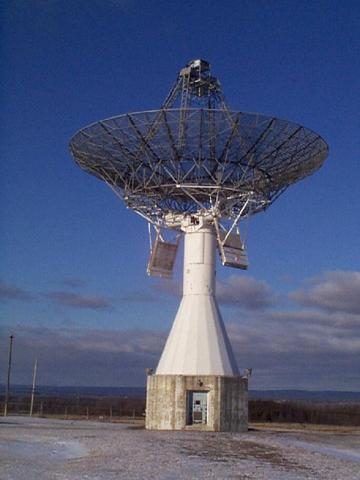
\includegraphics[width=0.2\linewidth]{images/ra.jpg}
\end{figure}
\note{Marcus is the Principal Investigator at SBRAC and also a contributor to the radiometer branch in GNURadio.  Although this branch is no longer maintained, he still answers questions about using radiometers with GNURadio}
\end{frame}

\begin{frame}
\frametitle{Related Works} 
Students at the University of Illinois and Grand Valley State University built a software defined radio to listen to emissions from Jupiter\cite{Behnke} by building their own RF section and using GNURadio for the software.  This software defined radio was built using an Analog Devices AD9460 and a Xilinx Spartan-3E-500 FPGA to build the SDR itself.

\begin{figure}\label{behnke}
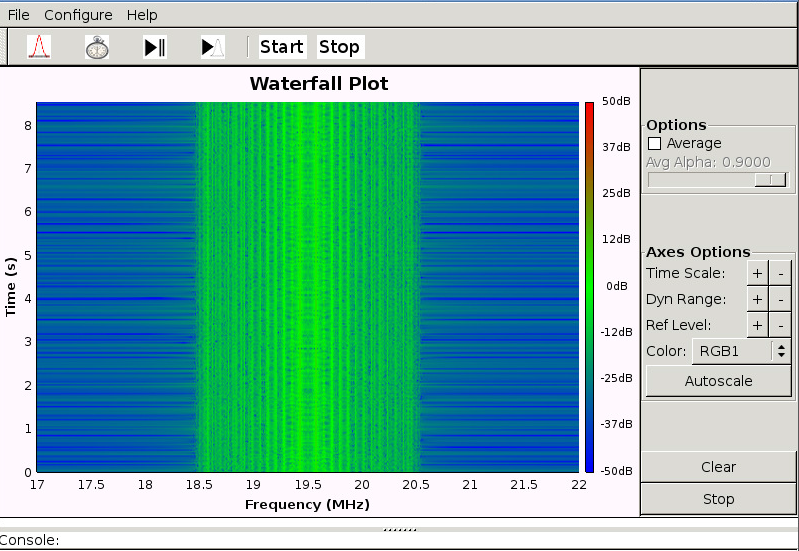
\includegraphics[width=0.5\linewidth]{images/behnke_GUI.png}
\end{figure}
\note{While the students in this paper built their own hardware, GNURadio was still used to develop the software.  Another goal of this project was to produce a low cost solution using GNURadio.}
\end{frame}
%---------------------------------------
\section{Radiometer Theory of Operation}
\subsection{Traditional Radiometer}
\begin{frame}
\frametitle{General Theory}
\begin{block}{Traditional Radiometer}
The primary goal of a radiometer is to measure power.  While that statement sounds easy, there are in fact many factors that go in to how well a radiometer can measure the power it sees.  A better statement would be that a radiometer's primary goal is to accurately measure power within a certain degree of accuracy.  In order to accurately and within a high degree of precision measure power, a radiometer must take into account various factors such as the system noise, the bandwidth of the signal and the stability of the system as a whole. 
\end{block}

\begin{figure}\label{crookes}
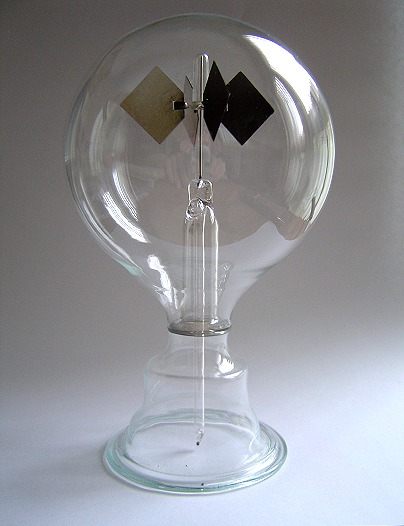
\includegraphics[width=0.15\linewidth]{images/Crookes_radiometer.jpg}
\end{figure}
\end{frame}

\begin{frame}
\frametitle{General Theory}
\begin{block}{Measuring power}
To measure power we begin with the noise signal coming from the antenna.  Our antenna is assumed to be looking at our target of interest and it is assumed that we can relate the antenna noise to the noise from the source.  It is often easier to refer to this noise as the brightness temperature.  Therefore the brightness temperature of the source can be related to the brightness temperature at the antenna.  We will refer to this brightness temperature as T$_{A}$\cite{Ulaby}.  

{\begin{figure}[h!tb] 
\centering
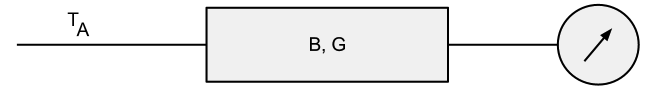
\includegraphics[width=\textwidth]{../Images/simple_rad.png}
\label{simplerad}
\end{figure}
}
\end{block}
\end{frame}

\subsection{RF Front End}
\begin{frame}
\frametitle{RF Front End Design}

The RF front end is one of the most critical components in a radiometer.  Although we have moved most of the functionality in to software with the SDR, we still need to amplify the signal.  Unlike other RF front ends though, we can use a fairly simple setup using 3 Low Noise Amplifiers (LNAs) and some basic filtering.  


\begin{figure}\label{AD_RFSIM}
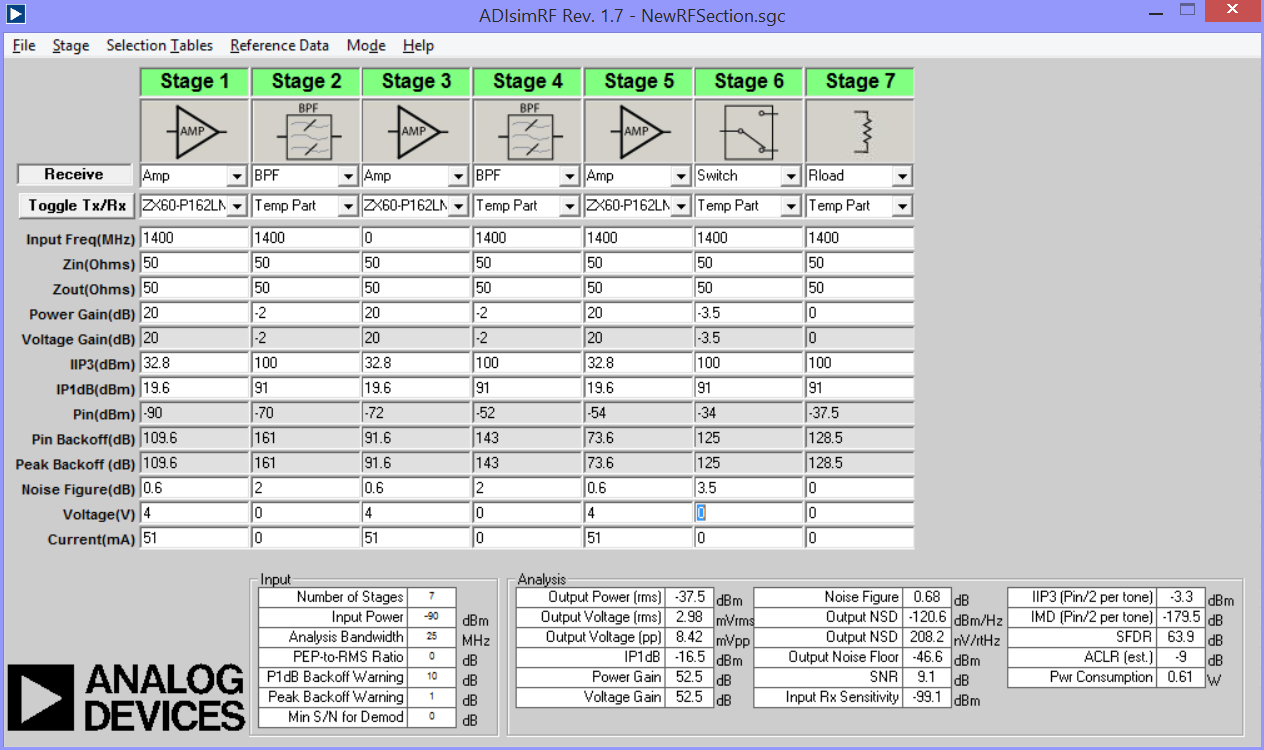
\includegraphics[width=0.6\linewidth]{images/RF_Front_end.png}
\end{figure}
\note{The image shown is Analog Devices program for analyzing gain, noise temperature and losses in a RF chain.  This program was used to analyze ours and other RF Front end systems.  The system shown is a simplified version of the RF front end used in testing.}
\end{frame}

\subsection{Software Defined Radio}
\begin{frame}
\begin{block}{SDR}
A software defined radio (SDR) is designed to mimic radio functions in software instead of using dedicated hardware.  A radiometer is a radio that can detect changes in power.  Therefore the SDR needs to be able to measure power coming from the source that we are looking at. 
\end{block}
\note{Software defined radios have been used in a number of applications, but usually related to communication systems.  Changes to modulation and encoding/decoding is very easy for a SDR and this is why SDRs have grown in recent years.  Use in remote sensing applications, as far as I know, is a relatively new application of SDRs.} 
\end{frame}
\subsection{SDR Radiometer}
%---------------------------------
\section{Comparison of Software Defined Radiometer to Traditional}
\subsection{SDR vs Traditional}
\begin{frame}
\frametitle{Comparison}
\begin{block}{Traditional Radiometer}
A traditional radiometer uses Low Noise Amplifiers, hardware based filters and a square-law detector to measure the power detected.  
\end{block}

\begin{block}{SDR Radiometer}
A software defined radiometer eliminates the filters and the square-law detector and replaces this with their mathematical equivalents that is emulated in software.   
\end{block}
\note{SDRs can filter in two ways.  First, by limiting the sampling rate we effectively put a bandwidth filter on the system.  Two, we can also filter by constructing a filter in software, although there is some cost with this option in terms of CPU and memory requirements on the system}
\end{frame}
\subsection{SDR vs Digital Radiometer}
\begin{frame}
\frametitle{Differences}
\begin{block}{Traditional Radiometer}
Most total power radiometers do not retain any frequency information, this information is lost and in most cases can not be recovered.
\end{block}

\begin{block}{SDR Radiometer}
Since we have both magnitude and phase information we can recreate the signal or manipulate it as needed.  This allows for more in-dept analysis such as RFI and also using Stokes parameters on the signal as well.  We therefore have more information without any additional hardware\cite{Ruf}.
\end{block}
\note{SDRs give us a lot more information to work with.  At the core of a radiometer, this information is not needed which is why it was often discarded.  However, several papers have now been written that bring to light the need for additional information in order to deal with known issues with radiometers such as interference or new methods for determining total power such as the Stokes method.  A key thing with a SDR radiometer is that in many ways it flexible enough to handle any future methods with either very little or no change in hardware.}
\end{frame}
%---------------------------------
\section{Implementation of a Software Defined Radiometer}
\begin{frame}
\frametitle{Implementation}
\begin{block}{Implementing a TPR}
A total power radiometer in software requires us to extract the magnitude (or amplitude) information from the I/Q data captured.  This is equivalent to what a square-law detector does in determining the power measured.
\end{block}
\note{Unlike an analog radiometer, the magnitude information is there and a simple squaring gives us total power.  A square-law detector however has to do just that, it detects the power and then extracts that as a voltage.}
\end{frame}
\subsection{Power detection/Square-law detector}
\begin{frame}
\frametitle{Implementation}
\begin{block}{Implementing a TPR}
For the SDR, the incoming signal is sampled and converted to I/Q values.  The I/Q values represent the amplitude and phase information of the signal.  In GNURadio we are then able to square these values within software.  This block in GNURadio mathematically performs the following:

\begin{equation}\label{sumIQ}
I^2+Q^2 = P_{out}
\end{equation}
\end{block}
\end{frame}
\subsection{Filtering}
\begin{frame}
\frametitle{Filtering}
Filtering requirements in a software defined radio is different from a hardware based or traditional radiometer.
\begin{itemize}
\item The bandwidth setting of the SDR only samples data within that bandwidth
\item Additional filters can be added at a cost of additional processing requirements
\item Because filtering is a simple software change, filters can be added and removed with no additional hardware
\end{itemize}

\end{frame}
\subsection{IIR as an integrator}
\begin{frame}
\frametitle{Integration}
The data we get from these power measurements fluctuate very quickly.  We want to smooth out or filter this data by integrating this over time.  In a traditional radiometer a hardware integrator is often used.  In software, we can use an Infinite Impulse Response (IIR) filter as an integrator.
\end{frame}
\begin{frame}
\frametitle{IIR as an integrator implementation}
\begin{block}{IIR and RC filter}
It can be seen that an IIR filter can have the same frequency response as we would expect from an analog RC filter.  As our sampling rate approaches infinity, the approximation gets closer to the original response from the analog RC circuit.  
\end{block}
\begin{equation}\label{final_IIR_RC}
y_n=\frac{T}{T+RC}x_n+\frac{RC}{T+RC}y_{n-1}
\end{equation}
\end{frame}

\subsection{GNURadio Blocks}
\begin{frame}
\frametitle{Implementation}

Implementation of a total power radiometer in software 

\begin{figure}\label{GNURadio_Block}
\includegraphics[width=9cm]{images/GNURadio_Block_tpr.png}
\end{figure}

\end{frame}

\subsection{GNURadio Controls}
\begin{frame}
\frametitle{GNURadio Controls}
GNURadio exposes GUI controls through wxGUI which allows us to implement a GUI system
\begin{figure}\label{GNURadio_GUI}
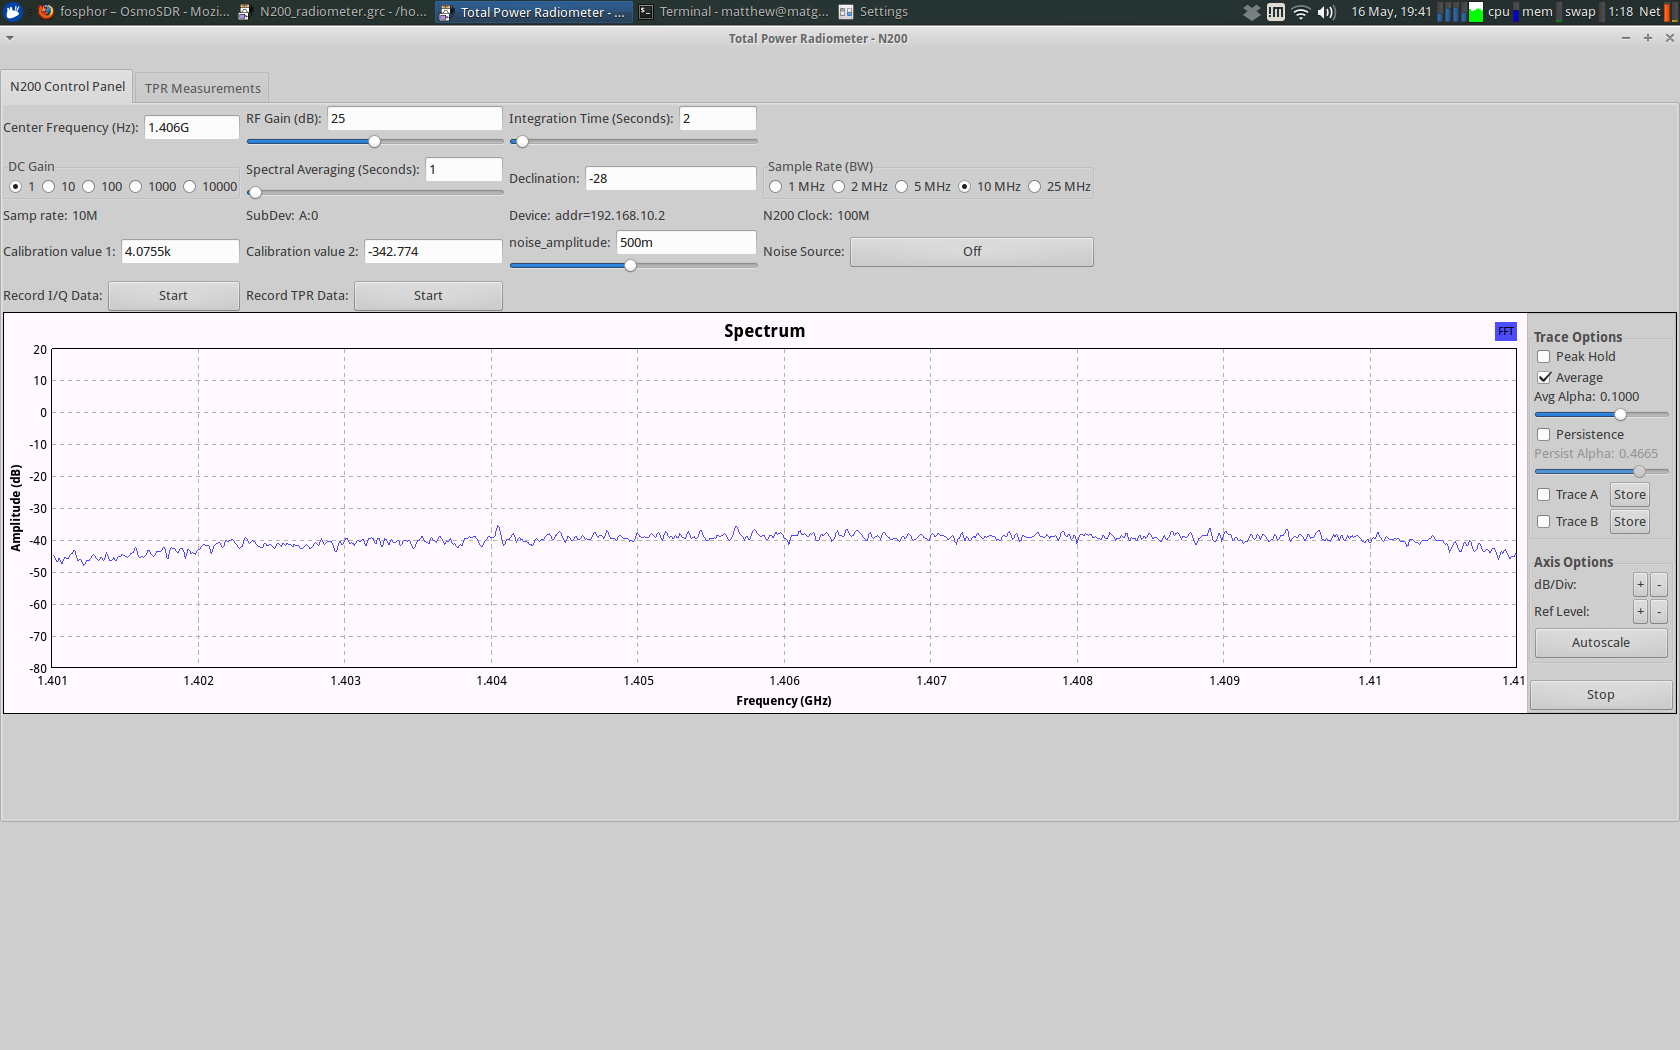
\includegraphics[width=10cm]{images/radiometer_gui.png}
\end{figure}
\note{The controls allow us to control a number of key features of the radiometer.  This includes bandwidth or sampling rate, the frequency, integration time and also the filter.}
\end{frame}

\subsection{GNURadio Display}
\begin{frame}
\frametitle{GNURadio Display}
As well as controls, we can also display information such as spectrum, total power and even a calibrated result.
\begin{figure}\label{GNURadio_GUI}
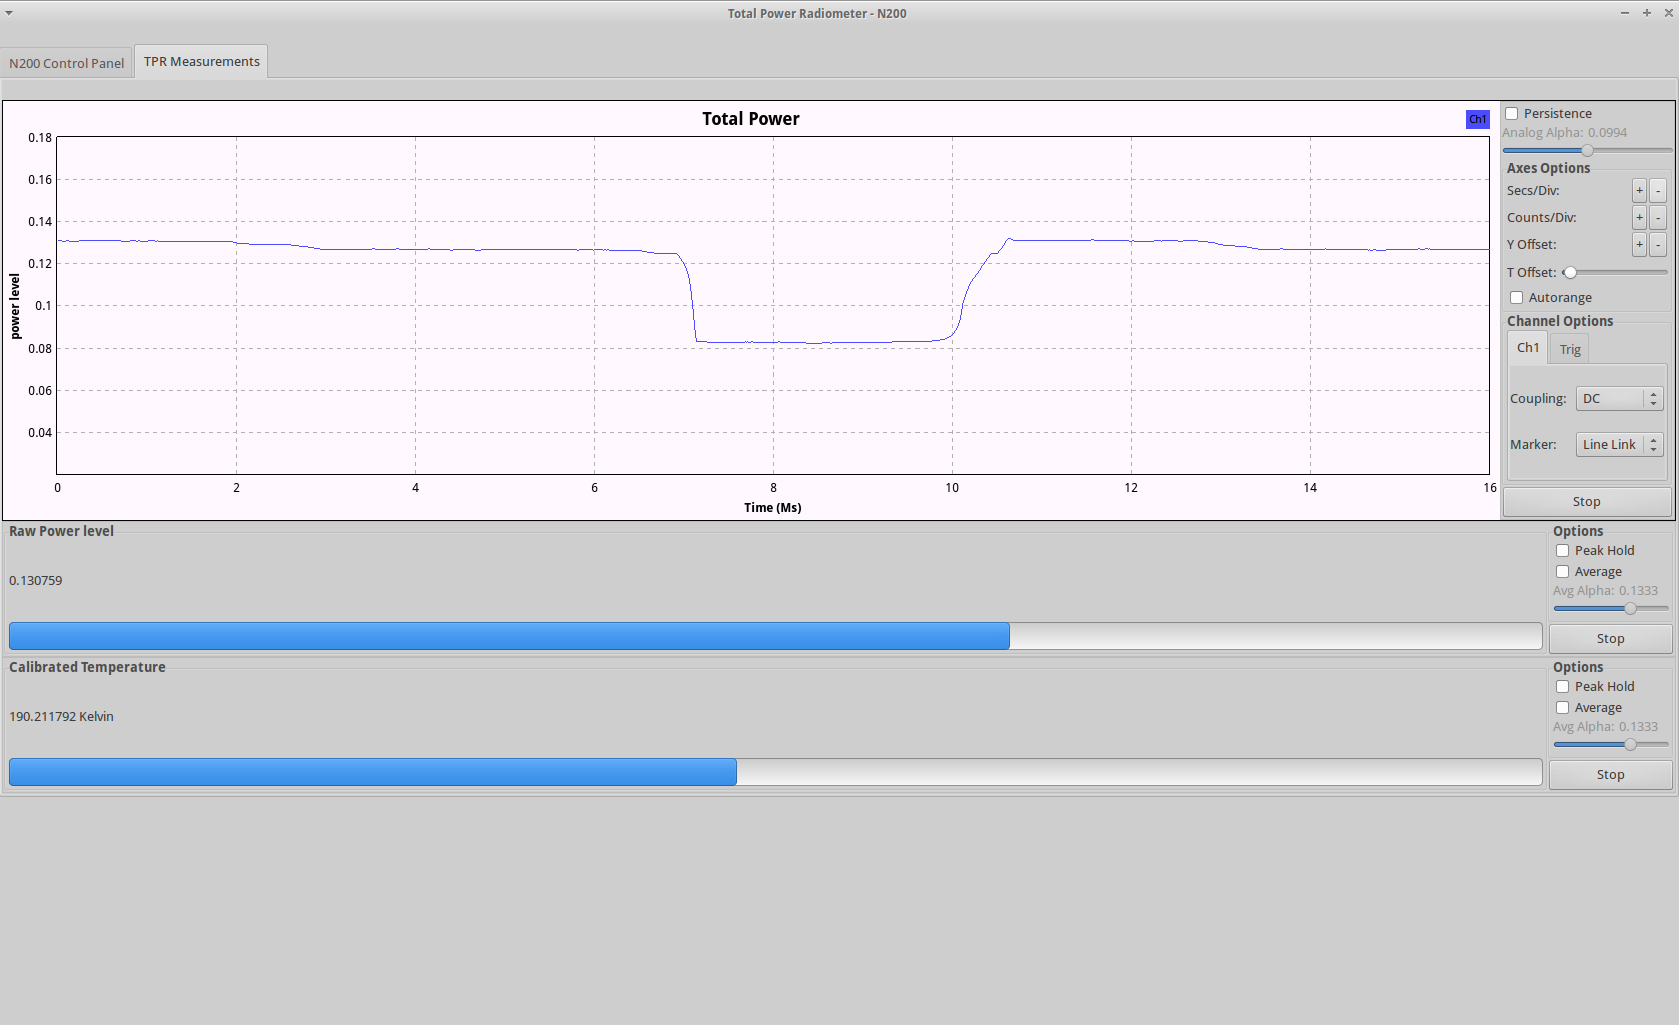
\includegraphics[width=10cm]{images/Lab1_TPR_at_end_exp.png}
\end{figure}
\note{The display can show both frequency information as well as total power.  Additional information such as calibrated noise temperature can also be shown}
\end{frame}
%-----------------------------
\section{Evaluation and Experimental Setup}
%-----------------------------
\section{Performance}
\subsection{Stability}
\begin{frame}
\frametitle{Stability}

Stability testing was accomplished by placing the matched load into a constant temperature bath and looking at amount of change over time.  A 4 hour soak test was done using Liquid Nitrogen.
\begin{figure}\label{calib_lab1}
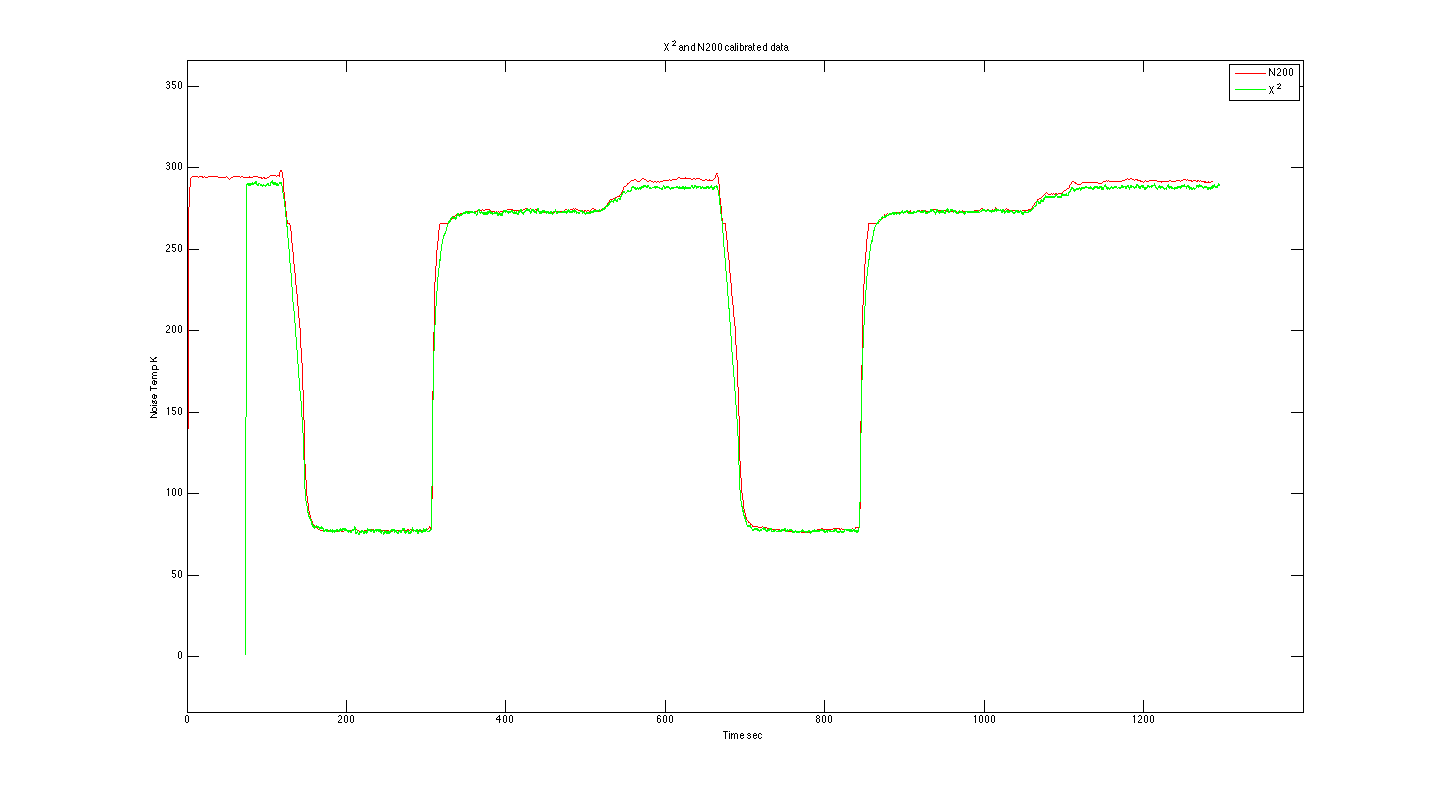
\includegraphics[width=1.0\linewidth]{images/lab1_both_calib.png}
\end{figure} 
\end{frame}
\subsection{Sensitivity}
\begin{frame}
\frametitle{Performance}
\begin{block}{Sensitivity}
The ability of a radiometer to detect these small changes is the radiometer's sensitivity, or the standard deviation of the output signal from the radiometer.  This sensitivity is also referred to as the Noise Equivalent $\Delta$ Temperature or NE$\Delta$T. 

\begin{equation}\label{NEAT}
NE\Delta T=\frac{T_{A}+T_{N}}{\sqrt{\beta * \tau}}
\end{equation}
\end{block}
\end{frame}
\subsection{Accuracy}
\begin{frame}
\frametitle{Performance}
\begin{block}{Accuracy}
blah blah blah
\end{block}
\end{frame}

%-------------------------------

\section{Results and Analysis}
\begin{frame}
\frametitle{Experimentation}
To verify that a software defined radio based radiometer can perform the same or better as a traditional radiometer, experiments were run to compare data captured from the SDR and data collected from a square-law detector, typically used to detect power in radiometers.  

In addition, we also wanted to test how a SDR can perform better than most traditional radiometers since frequency information is retained.  To do this, we tested with the ability to filter out an unwanted signal and compared the results.
\end{frame}
\subsection{SDR compared with square-law detector}
\begin{frame}
\frametitle{LN2 Tests}
Calibration and testing of the radiometer was conducted by using two reference temperature points.  The two points selected was Liquid Nitrogen at 77 K and Ice Water at 273.15 K. 

\begin{figure}\label{LN2_stability}
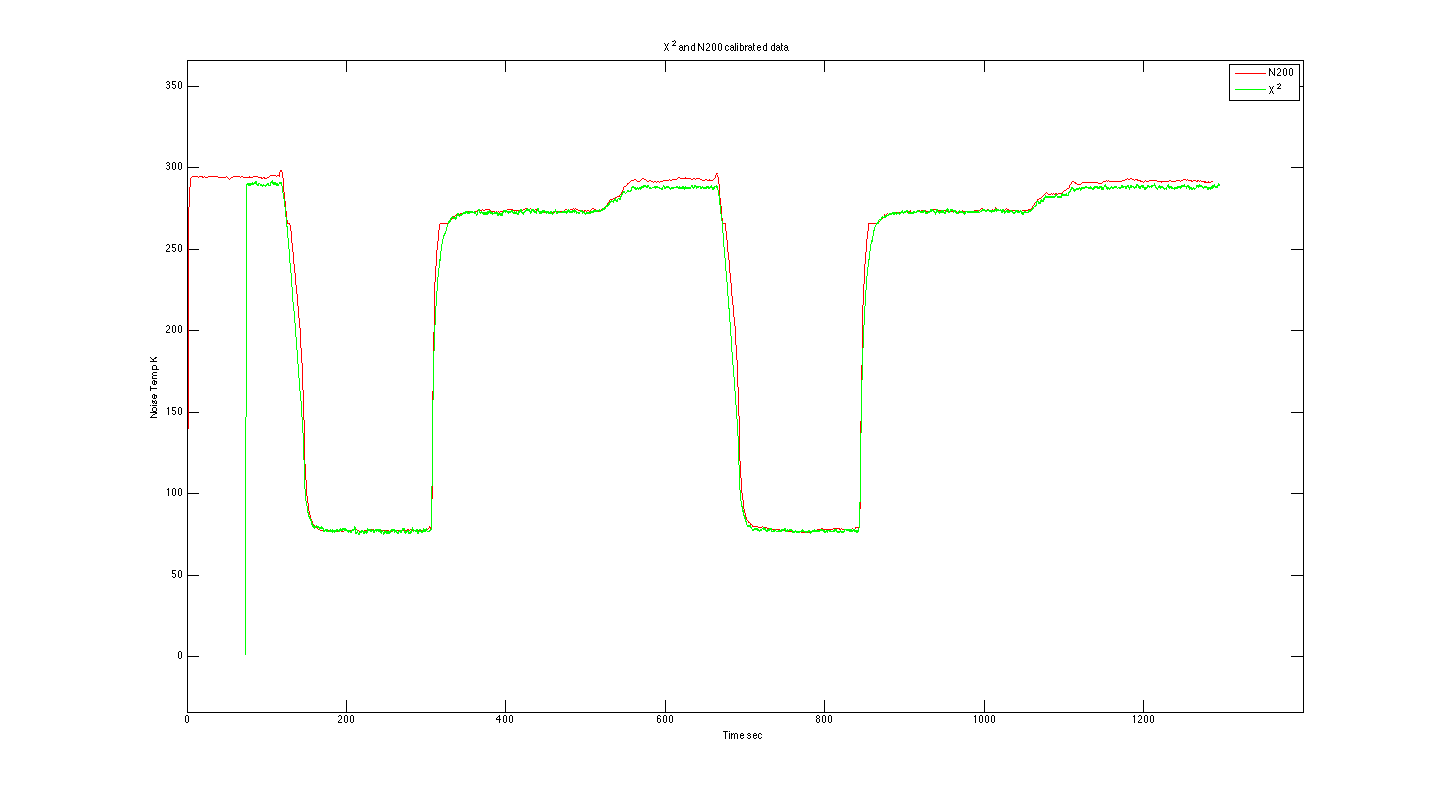
\includegraphics[width=1.0\linewidth]{images/lab1_both_calib.png}
\end{figure} 
\end{frame}
\subsection{Filtering an unwanted signal}
\begin{frame}
\frametitle{Unwanted signal filter}
Another experiment was conducted, but this time with a signal injected that interferes with the radiometer.
\begin{figure}\label{filter_signal}
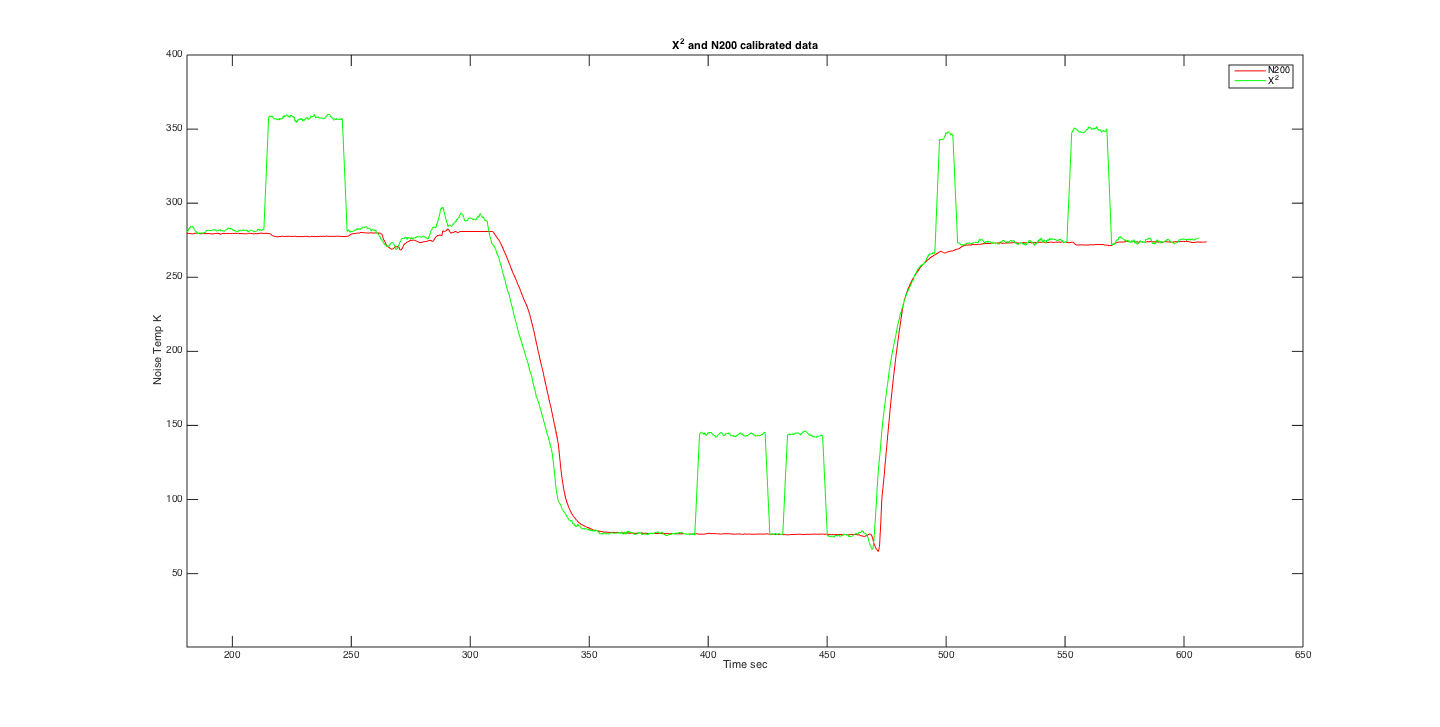
\includegraphics[width=1.0\linewidth]{images/moneyshot.png}
\end{figure} 
\end{frame}
%---------------------------------
\section{Conclusion and Future Work}
\begin{frame}
\frametitle{Conclusion}
\begin{block}{Final Thoughts}
In this thesis we have shown that an off the shelf SDR can be used to perform as a radiometer.  Using a SDR has several advantages such as a more flexible system and can result in a less expensive system.  Since a SDR offers high flexibility, changes to the system can be done very quickly and helps in future proofing the system.  
\end{block}
\end{frame}
\section{Future Work}
\begin{frame}
\frametitle{Future Work}
\begin{block}{Future Items}
\begin{itemize}
\item Make improvements to the ISU RF Front End
\note<1>{Fix issues with SWR and interference}
\item Rebuild the ISU radiometer
\note Replacing the Rabbit uC with PIC32
\item Correlation
\item Noise Injection
\item Stokes parameters
\end{itemize}
\end{block}
\end{frame}

\section{References}
% Beamer does not support BibTeX so references must be inserted manually as below
\begin{frame}
\frametitle{References}
\footnotesize{
\begin{thebibliography}{99}
\bibitem[Skou, 2006]{Skou} Niels Skou and David Le Vine (2006)
\newblock Microwave Radiometer Systems Design and Analysis
\newblock \emph{Artech House}

\bibitem[Ulaby, 1981]{Ulaby} F. T. Ulaby, R. K. Moore and A. K. Fung (1981)
\newblock Microwave Remote Sensing
\newblock \emph{Artech House}

\bibitem[Leech, 2007]{Leech2007} Marcus Leech and David Ocame (2007)
\newblock A year of Gnu Radio and SDR astronomy: experience, practice and observations
\newblock \emph{\url{http://www.sbrac.org/documents/gnuradio_at_one_year_20070401.doc}}

\bibitem[Behnke, 2013]{Behnke} Behnke, P. and Soberal, D. and Bredeweg, S. and Dunne, B. and Sterian, A. and Furton, D. (2013)
\newblock Senior capstone: A software defined radio design for amateur astronomy
\newblock Interdisciplinary Engineering Design Education Conference (IEDEC), 2013 3rd

\bibitem[Ruf, 2010]{Ruf} Ruf, C. and Gross, S. (2010)

\newblock Digital radiometers for earth science

\newblock Microwave Symposium Digest (MTT), 2010 IEEE MTT-S International

\end{thebibliography}
}
\end{frame}
%------------------------------------------------

\begin{frame}
\Huge{\centerline{The End}}
\end{frame}

%----------------------------------------------------------------------------------------
\begin{frame}
\Huge{\centerline{Extra Slides}}
\end{frame}
\section*{Extra Slides}

\begin{frame}
\begin{block}{Secondary goal}
A secondary goal was to use off the shelf components and components that are generally more accessible.  This would allow radiometers to be more accessible to a wider scope of researchers in this field.
\end{block} 

\begin{block}{Tertiary goal}
And finally a tertiary goal was to ensure that the system as a whole is fairly easy to use.  This ties to our secondary goal of making radiometers more accessible to a wider range of researchers and research topics.
\end{block}
\end{frame}

\begin{frame}
\begin{block}{Ideal Radiometer}
Figure on slide~\ref{simplerad} shows us an ideal radiometer.  That is a radiometer that has an input from the antenna, T$_{A}$, a known bandwidth denoted as B and a known gain denoted as G.  At the end of the block is the detector, which measures the power from the radiometer.
\end{block}
\end{frame}

\begin{frame}
\begin{block}{Bandwidth}
Only a certain selection of the radio spectrum is observed by the radiometer.  This is referred to as the bandwidth of the radiometer and is denoted as B or as $\beta$.  This bandwidth is then centered around a center frequency.  In our case, we center around 1.405 GHz as this falls in a protected frequency range often used for radiometry.  
\end{block}
\end{frame}

\begin{frame}
\begin{block}{Power}
The power coming from the antenna is amplified so it is easier to determine changes in the brightness temperature.  The overall gain of the radiometer system is referred to as G in this case.  Finally, we need to apply Boltzmann's constant, referred to as \textit{k}.  With these values, we can now compute the power the radiometer will see for an ideal radiometer.  This can be shown in equation~\ref{eq:power_rad_eq}

\begin{equation} \label{eq:power_rad_eq}
P=k*\beta*G*(T_{A})
\end{equation}
\end{block}

\end{frame}

\begin{frame}
\begin{block}{Noise}
However, since we do not have an ideal radiometer, we have another key component that needs to be addressed and that is the noise added to the system from the radiometer itself.  Most of the additional noise is from the Low Noise Amplifiers (LNA) that are used to increase the signal while attempting to keep the noise added to a minimum.  The Figure below shows the additional noise that is injected into the system.

{\begin{figure}[h!tb] 
\centering
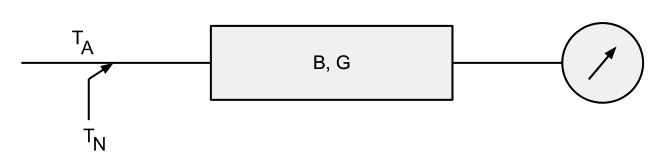
\includegraphics[width=\textwidth]{../Images/radiometer_noise_added.png}
\label{noiserad}
\end{figure}
}
\end{block}
\end{frame}

\begin{frame}
\begin{block}{Antenna Noise}
As it can be seen, this additional noise is added to the noise coming from the antenna source.  Therefore T$_{N}$ is added to T$_{A}$ and our final equation for the power measured is shown in equation~\ref{eq:final_power}.  

\begin{equation} \label{eq:final_power}
P=k*\beta*G*(T_{A}+T_{N})
\end{equation}
\end{block}
\end{frame}

\begin{frame}
\begin{block}{IIR Filter}
This signal will fluctuate rapidly and to improve the sensitivity of the radiometer we wish to integrate this signal.  A RC filter is analogous to an integrator where the R and C values determine our time constant and our integration time for the filter.  A SDR however operates in the digital domain at discrete intervals.  One type of filter that can be used in the Infinite Impulse Response (IIR) filter. 
\end{block}
\end{frame}

\begin{frame}
\begin{block}{RC Filter}
To begin with, we look at what an analog RC filter looks like. 

{\begin{figure}[h!tb] 
\centering
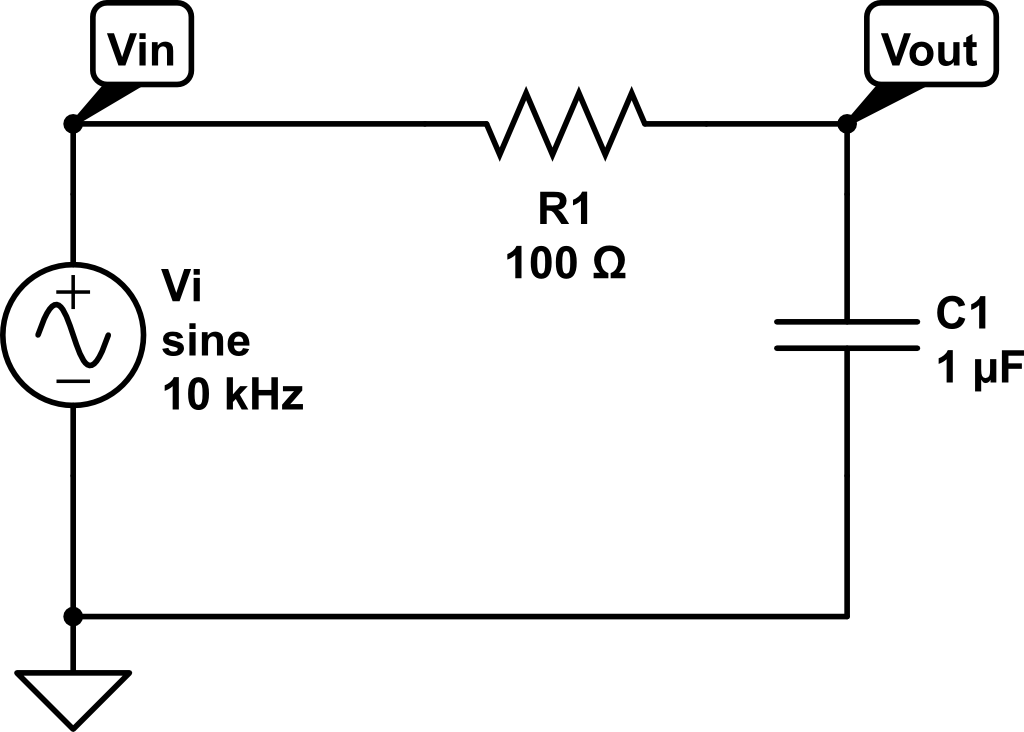
\includegraphics[width=7cm]{../Images/rc-circuit.png}
\label{rc_circuit}
\end{figure}
}
\end{block}
\end{frame}

\begin{frame}
\begin{block}{RC Filter Eqs}
This circuit can be represented by the following equation.
\begin{equation}\label{eq:rc_circuit_eq}
\frac{V_{in}-V_{out}}{R}=C\frac{dV_{out}}{dt}
\end{equation}
\end{block}
\end{frame}

\begin{frame}
\begin{block}{FIR Filter}
A Finite Impulse Response (FIR) filter is a digital filter that can take an impulse signal and decays to zero after a finite number of iterations.  This type of digital filter can be represented by the following equation:

\begin{equation}\label{IIR_yn}
y_n=\displaystyle\sum\limits_{i=o}^{P-1} c_ix_{n-i}
\end{equation}
\end{block}
\end{frame}

\begin{frame}
\begin{block}{IIR Filter}
An Infinite Impulse Response (IIR) filter is the same as the FIR filter, except that we add an additional summation term which feeds back the previous output.

\begin{equation}\label{IIR_sum}
y_n=\displaystyle\sum\limits_{i=o}^{P-1} c_ix_{n-i}+\displaystyle\sum\limits_{j=1}^{Q} d_jy_{n-j}
\end{equation}

It can be seen that a FIR filter is really a IIR filter except that $Q=0$.  
\end{block}
\end{frame}

\begin{frame}
\begin{block}{IIR and RC Filter}
To get a better understanding on how our digital IIR filter relates to our RC filter analog, we can look at the Fourier Transform and the relationship of the input to the output in the frequency domain.

\begin{equation}\label{Fourier}
H(f)=\frac{\displaystyle\sum\limits_{j=o}^{P-1} c_je^{-2\pi ijfT}}{1-\displaystyle\sum\limits_{k=1}^{Q} d_ke^{-2\pi ikfT}}
\end{equation}

Here $f$ is our frequency in Hz and $T$ is the time between samples in seconds.
\end{block}
\end{frame}

\begin{frame}
\begin{block}{Link between RC and IIR}
We now want show the link between our analog RC circuit and the IIR filter.  Looking at equation \ref{eq:rc_circuit_eq}, which represents the differential equation relating the input voltage $V_{in}$ to the output voltage $V_{out}$, we can substitute for input and output of our IIR filter.  Since we are now in the time domain, we need to define what $T$ is.

\begin{equation}\label{Sample}
T=time between samples=\frac{1}{sampling rate}
\end{equation}
\end{block}
\end{frame}

\begin{frame}
\begin{block}{input voltage to IIR}
We can now relate our input voltage to the input to our IIR filter and the output voltage to the output of our IIR filter.

\begin{equation}\label{IIRxn}
x_n=v_{in}(nT)
\end{equation}

\begin{equation}\label{yn_out}
y_n=v_{out}(nT)
\end{equation}
\end{block}
\end{frame}

\begin{frame}
\begin{block}{Rewrite difference eq}
We can now rewrite our difference equation with $x_n$ and $y_n$.

\begin{equation}\label{diff_xn}
\frac{x_n-y_n}{R}=C\frac{y_n-y_{n-1}}{T}
\end{equation}

Now, we can solve for $y_n$ which results in our final equation for showing how a IIR filter is related to an RC filter.

\begin{equation}\label{IIR_RC}
y_n=\frac{T}{T+RC}x_n+\frac{RC}{T+RC}y_{n-1}
\end{equation}
\end{block}
\end{frame}

%\begin{frame}
%\begin{block}{IIR and RC filter}
%It can be seen that an IIR filter can have the same frequency %response as we would expect from an analog RC filter.  As our %sampling rate approaches infinity, the approximation gets closer to %the original response from the analog RC circuit.  
%
%\end{block}
%\end{frame}

\begin{frame}
\frametitle{Multiple Columns}
\begin{columns}[c] % The "c" option specifies centered vertical alignment while the "t" option is used for top vertical alignment

\column{.45\textwidth} % Left column and width
\textbf{Heading}
\begin{enumerate}
\item Statement
\item Explanation
\item Example
\end{enumerate}

\column{.5\textwidth} % Right column and width
Lorem ipsum dolor sit amet, consectetur adipiscing elit. Integer lectus nisl, ultricies in feugiat rutrum, porttitor sit amet augue. Aliquam ut tortor mauris. Sed volutpat ante purus, quis accumsan dolor.

\end{columns}
\end{frame}


\begin{frame}
\frametitle{Table}
\begin{table}
\begin{tabular}{l l l}
\toprule
\textbf{Treatments} & \textbf{Response 1} & \textbf{Response 2}\\
\midrule
Treatment 1 & 0.0003262 & 0.562 \\
Treatment 2 & 0.0015681 & 0.910 \\
Treatment 3 & 0.0009271 & 0.296 \\
\bottomrule
\end{tabular}
\caption{Table caption}
\end{table}
\end{frame}


\begin{frame}[fragile] % Need to use the fragile option when verbatim is used in the slide
\frametitle{Verbatim}
\begin{example}[Theorem Slide Code]
\begin{verbatim}
\begin{frame}
\frametitle{Theorem}
\begin{theorem}[Mass--energy equivalence]
$E = mc^2$
\end{theorem}
\end{frame}\end{verbatim}
\end{example}
\end{frame}


\end{document} 